\documentclass[12pt]{article}
%\documentclass{nature}

% Including pdf figures
\usepackage{graphicx}
\graphicspath{ {../Plots/} }
\usepackage{pdfpages}
%really place a figure in a location
\usepackage{float}
%Overrun caption
\usepackage[CaptionAfterwards]{fltpage}
% Math stuff
\usepackage{amsmath}
% Bibliographies
\usepackage[numbers]{natbib}
\bibpunct{(}{)}{,}{a}{}{;} 

\usepackage[flushleft]{threeparttable}

\usepackage[font={scriptsize}]{caption}

\usepackage{lineno} %gives line numbers with \lineno command

\usepackage{setspace}
\onehalfspace

\begin{document}

\title{Gametic Selection, Sex Ratio Bias, and Transitions Between Sex Determination Systems}
\author{Michael F Scott$^{*1}$ and Matthew M Osmond$^{*2}$, and Sarah P Otto$^2$}
\date{}
\maketitle
\noindent
$*$ These authors contributed equally to this work

\noindent
$^1$ Department of Botany, University of British Columbia, \#3529 - 6270 University Boulevard, Vancouver, BC, Canada V6T 1Z4

\noindent
$^2$ Department of Zoology, University of British Columbia, \#4200 - 6270 University Boulevard, Vancouver, BC, Canada V6T 1Z4

\noindent
email: mfscott@biodiversity.ubc.ca, mmosmond@zoology.ubc.ca

\noindent
Contributions: 

\newpage
\linenumbers
\modulolinenumbers[2]

\begin{abstract}
Sex determination systems are remarkably dynamic; many studied taxa display transitions between sex-determining genes across chromosomes or the evolution of new sex-determining systems. 
%Predominant theories in which new sex-determining systems are favoured by selection involve sex ratio selection or fitness differences between sexes (e.g., sexually antagonistic selection). 
Here, we utilize population genetic models to study the spread of novel sex-determiners in systems with 
%a period of selection during the haploid stage produced by one sex, e.g., pollen or sperm competition. 
haploid gametic selection, e.g., pollen or sperm competition.
Haploid selected loci experience a form of sex-specific selection when gametic competition occurs predominantly among haploids produced by one sex (e.g.,  pollen competition).
This can cause sex ratios at birth to become biased as sex ratios are determined by the fertilization success of X- versus Y-bearing pollen/sperm (or Z- versus W-bearing eggs). 
%We find that the evolution of sex determination systems where mothers determine sex at birth (e.g., environmental sex determination where sex is determined at birth) is influenced by classic Fisherian sex ratio selection. {\color{red}(Maybe not true???)}
%However, notably, we find that the spread of new genetic sex determination systems is not affected by sex ratio biases that are caused by gametic selection because sex ratios become biased after parental provisioning has occurred (even if pollen/sperm competition occurs within the mother). 
Notably, we find that the spread of new genetic sex determination systems is not affected by sex ratio biases that are caused by gametic selection because sex ratios become biased after parental provisioning has occurred, even if pollen/sperm competition occurs within the mother (e.g., pollen competition in stigma). 
In addition, we find that linkage of an ancestral sex chromosome to a locus under haploid selection can favour transitions between male and female heterogamety (e.g., XY to ZW), which is not the case for any forms of diploid sex specific selection (e.g., sexually antagonistic selection).
During these transitions, new sex-determining alleles spread despite breaking up favourable associations that build up between ancestral sex-determining loci and selected loci, reducing population mean fitness. 
Furthermore, a period of selection among haploids can favour the stable maintenance of polymorphic sex determination systems. 
Thus, our models offer several new insights to be explored as information about sex determination in non-model taxa accumulates.

%[Approx 320 words]
\end{abstract}

\newpage

\section*{Introduction}

%CHECK THROUGHOUT: use of sex-determination SYSTEMS versus MECHANISMS. 

Animals and angiosperms exhibit extremely diverse sex determination systems \citep[reviewed in][]{Bull:1983vi,Charlesworth:2010it,Beukeboom:2014vb,Bachtrog:2014bx}. 
Among species with genetic sex determination of diploid sexes, some taxa have heterogametic males (XY) and homogametic females (XX), including %non-monotreme? 
mammals and most dioecious plants \citep{Ming:2011iy}; whereas other taxa have homogametic males (ZZ) and heterogametic females (ZW), including Lepidoptera and birds. 
Within several taxa, the chromosome that harbours the master sex-determining region changes. 
For example, transitions of the master sex-determining gene between chromosomes or the evolution of new master sex-determining genes have occurred in Salmonids \citep{Li:2011fm,Yano:2012di}, Diptera \citep{Vicoso:2015hf}, and \textit{Oryzias} \citep{Myosho:2012fv}.
%Presentation at evolution found neo sex chromosome in birds, doesn't seem to be published or bioRxiv yet (consider pers com.), title: A previously unknown neo-sex chromosome mediates plumage divergence and speciation in hybridizing birds Jason Sardell; Elizabeth Cooper; J. Albert C. Uy. I wonder if this is actually a fusion event though?
In addition, many gonochoric/dioecious clades with genetic sex determination exhibit transitions between male (XY) and female (ZW) heterogamety, including lizards \citep{Ezaz:2009tk}, eight of 26 teleost fish families \citep{Mank:2006bt}, true fruit flies \citep[Tephritids,][]{Vicoso:2015hf}, amphibians \citep{Hillis:1990gu}, the angiosperm genus \textit{Silene} \citep{Slancarova:2013dq}, Coleoptera and Hemiptera \citep[][plate 2]{Beukeboom:2014vb}.
Indeed, in some cases, both male and female heterogametic sex determination systems can be found in the same species, as exhibited by some cichlid species \citep{Ser:2010iq} and \textit{Rana rugosa} \citep{Ogata:2007jm}.
In addition, multiple transitions have occurred between genetic and environmental sex determination systems, e.g., in reptiles and fishes \citep{Conover:1987in,Mank:2006bt,Pokorna:2009ui,Ezaz:2009tk,Pen:2010kk,Holleley:2015hc}.

%NOTE: ``Bull & Charnov (1977) hypothesized that a new sex-determining gene can rapidly increase and become fixedin a population if it is linked to a gene with high adaptivevalue, and finally cause a change of the heterogametic sex.'' The Bull and Charnov paper is also the one in which the set of neutral equilibria between XY and ZW are identified (where sex ratios are equal)
%NOTE: Vuilleumier et al. 2007 also find polymorphic sex determination can be stable.

%For example, closely related species in the Medaka lineage (cite Takenhana et al. 2008) and Tilapiinae (cite Lee et al 2004, Cnaani et al 2008), citations in Beukeboom. 

%\textcolor{red}{Brief description of sex ratio adjustment and sexual antagonism theories:}

Predominant theories in which new sex determination systems are favoured by selection involve fitness differences between sexes (e.g., sexually antagonistic selection) or sex ratio selection.
%\citet{Bull:1977wt} shows that direct selection on new sex determination loci can allow them to spread and switch between male and female heterogamety. 
\citet{vanDoorn:2007eu,vanDoorn:2010hu} show that new sex determination loci can be favoured if they arise in close linkage with a locus that experiences sexual antagonism. 
For example, linkage allows favourable associations to build up between a male-beneficial allele and a neo-Y chromosome. 
Such associations can favour a new master sex-determining gene on a new chromosome \citep{vanDoorn:2007eu} and can also favour a transition between male and female heterogamety \citep[e.g., a ZW to XY transition,][]{vanDoorn:2010hu}.
However, any sexually-antagonistic loci that are linked to the ancestral sex-determination locus will develop similar, favourable associations and select against the spread of a new sex-determination system. 

It has been suggested that sex ratio selection could be a particularly important force driving transitions between sex-determining systems \citep[Chapter 7]{Beukeboom:2014vb}. 
For example, flexible sex determination systems may be favoured in order to exploit local environmental conditions that are optimal for males or females, which creates locally biased sex ratios \citep{Charnov:1977tx,Werren:1984tl,Pen:2010kk}. 
In addition, feminizing mutations may invade when female biased sex ratios are favoured due to selection among demes \citep{Wilson:1981vm,Vuillleumier:2007bh}. 
In other situations, sex ratio selection may favour transitions in order to restore equal sex ratios. 
For example, \citet{Kozielska:2010vm} consider systems in which the ancestral sex chromosomes experience meiotic drive (e.g., where driving X or Y chromosomes are inherited disproportionately often), which causes sex ratios to become biased \citep{Hamilton:1967ts}. 
They find that new, unlinked sex-determining loci (masculinizing or feminizing mutations, i.e., neo-Y or neo-W loci) can then spread, restoring an even sex ratio. 

%\textcolor{red}{We add haploid selection:}

Here, we use mathematical models to find the conditions under which new sex determination systems are favoured by selection when there is a period of selection among haploid gametes/gametophytes. 
Selection among haploid genotypes is thought to occur primarily among pollen/sperm, which can compete whenever there are more pollen/sperm than required for fertilization \citep{Mulcahy:1996ha,JOSEPH:2004haa}. 
Haploid selection may be particularly common in plants, in which 60-70\% of all genes are expressed in the male gametophyte and these genes exhibit stronger signatures of selection than random genes \citep{Borg:2009jpa,Arunkumar:2013iq,Gossmann:2014dua}.
In addition, artificial selection pressures applied to male gametophytes cause the frequency of resistant alleles to increase \citep[e.g.,][]{Hormaza:1996cv,Ravikumar:2003uo,Hedhly:2004iv,Clarke:2004ir}. 
A smaller (but non-negligible) proportion of genes are thought to be expressed and selected in animal sperm, although precise estimates are uncertain \citep{Zheng:2001fi,JOSEPH:2004haa,Vibranovski:2010et}.
%\textcolor{red}{add something about meiotic drive here?}  

There are various ways in which a period of haploid selection could influence transitions between sex determination systems. 
Firstly, if we assume that haploid selection at any particular locus predominantly occurs in one sex (e.g., pollen/sperm competition), then such loci experience a form of sex-specific selection. 
In this respect, we might expect that haploid selection might affect transitions between sex determination systems in a similar manner to sex-specific diploid selection \citep[as explored by][]{vanDoorn:2007eu,vanDoorn:2010hu}. 
That is, new masculizing mutations (neo-Y chromosomes) could be favoured via linkage associations with alleles that are beneficial in pollen/sperm. 
However, sex ratios can also become biased if there is linkage between the sex-determining region and a locus that harbours genetic variation in haploid fitness. 
For example, differences in fitness between X- and Y-bearing pollen tubes can cause the sex ratio among seeds to become biased when there is pollen competition \citep{Lloyd:1974tz,Conn:1981uw,Stehlik:2005ul,Stehlik:2006to,Field:2012fd,Field:2013cc}.
It is not immediately clear how the spread of new sex determination systems would be influenced by the combination of sex ratio biases and favourable associations between haploid selected loci and sex-determining regions. 

Surprisingly, our models show that haploid selection influences the evolution of new sex determination systems in a way that is distinct from both diploid sex-specific selection and sex ratio selection. 
We find that new genetic sex determination systems are not affected by any sex ratio biases caused by associations between sex-determining regions and haploid selected loci. 
In addition, we find that associations that build up between an ancestral sex-determining locus and a haploid-selected locus can favour transitions between male and female heterogamety (e.g., a neo-W allele arising at a previously autosomal locus spreads in an ancestrally XY system), despite the fact that these ancestral associations were built up by selection. 
This does not occur in models that do not include haploid selection. 

\textcolor{red}{NOTE RE: DRIVE. I expect drive (that occurs specifically in one sex, e.g., during spermatogenesis) to behave almost exactly like haploid selection. That is, I think that a XY-linked driver that is maintained by selection (e.g., because it causes sterility when homozygous, which is common in known drive systems) will only favour invasion of a more tightly linked neo-Y (worsening sex ratio biases) and could favour invasion of a neo-W. This may run counter to generic expectations from new sex chromosome systems evolving to balance the sex ratio. So, do you think it would significantly enhance the paper to model drive explicitly or just discuss it as being similar???}

{\color{blue} 
FOR RESULTS?

FROM PREVIOUS PAPER:
The maintenance of polymorphism at loci that experience sex specific selection in both haploid and diploid phases was considered by Immler et al. \cite{Immler:2012tl}, demonstrating that polymorphisms can be maintained by sexually antagonistic selection or overdominance as well as by conflicting selection pressures in haploids and diploids (haploid-diploid conflict or ploidally antagonistic selection) or a combination of these selective regimes.  
}


%%%%%%%%%%%%%%%%%%%%%%%%%%
\section*{Model}
%%%%%%%%%%%%%%%%%%%%%%%%%

%genetic system
We consider the transition between ancestral and novel sex determination systems using a three locus model.
Locus \textbf{X} is the ancestral sex-determining region, with alleles $X$ and $Y$ (or $Z$ and $W$).
Locus \textbf{A} is a locus under selection, with alleles $A$ and $a$.
Locus \textbf{M} is a novel sex-determining region, at which the null allele ($M$) is initially fixed in the population such that sex of zygotes is determined by the genotype at the ancestral sex-determining region, \textbf{X} ($XX$ become females and $XY$ become males, or $ZW$ become females and $ZZ$ become males). 
To evaluate the evolution of new sex-determination systems, we consider the invasion, fixation, maintenance, and/or loss of novel sex-determining alleles ($m$) at the \textbf{M} locus. 
%We only do invasion analytically though (is this sentence still ok?)
We assume that the \textbf{M} locus is dominant over the \textbf{X} locus such that zygotes with at least one $m$ allele develop as females with probability $k$ and as males with probability $1-k$, regardless of the \textbf{X} locus genotype.
With $k=0$, the $m$ allele is a masculinizer (i.e., a neo-Y) and with $k=1$ the $m$ allele is a feminizer (i.e., a neo-W).
With intermediate $k$, the $m$ allele confers environmental sex determination such that zygotes develop as females in a proportion ($k$) of the environments they experience. 
Finally, we also analyze a model of maternally-controlled environmental sex-determination (ESD), where mothers with at least one $m$ allele produce daughters with probability $k$. 

%life-cycle
In each generation, we census the genotype frequencies in male and female gametes/gametophytes (hereafter gametes) before haploid competition (see Sup.\ Mat. for recursion equations). 
First, competition occurs among male gametes (sperm/pollen competition) and among female gametes (egg/ovule competition). 
Selection during haploid competition depends on the \textbf{A} locus genotype, fitnesses are $w_{A}^m$ and $w_{a}^m$ for male gametes and $w_{A}^f$ and $w_{a}^f$ for female gametes, see table \ref{tab:fitnesstable}. 
Random mating then occurs between male and female gametes.
The resulting zygotes develop as males or females, depending on their genotypes at the \textbf{X} and \textbf{M} loci (and the \textbf{M} genotype of their mother in the case of maternal control) as described above.
Diploid males and females then experience selection, male fitness is given by $w_{h}^{m}$ and female fitness by $w_{h}^{f}$, where $h$ is the genotype at the \textbf{A} locus ($h \in AA, Aa, aa$).  
%Diploids compete with others of the same sex, where selection depends on the sex of the individual and its genotype at the \textbf{A} locus.
The next generation of gametes are then produced by meiosis, during which recombination and sex-specific meiotic drive can occur. 
Recombination occurs between loci \textbf{X} and \textbf{A} with probability $r$, between loci \textbf{A} and \textbf{M} with probability $R$, and between loci \textbf{X} and \textbf{M} with probability $\chi$.
Therefore, any order of the loci can be modelled with appropriate choices of $r$, $R$, and $\chi$ (see Table \ref{tab:chisubstitutions}). 
Males/females that are heterozygous at the \textbf{A} locus experience meiotic drive; $Aa$ heterozgotes of sex $d$ produce gametes bearing allele $A$ with probability $\alpha^d$. 
Thus, the \textbf{A} locus can experience sex-specific haploid competition, diploid selection and/or meiotic drive. 

\begin{table}[ht]
\centering
\smallskip
\caption{Fitness of different genotypes in sex $d$}
\begin{tabular}{l c }
\hline\hline
  Genotype & Fitness during haploid competition \\ [0.5ex] \hline
  A & $w_{A}^d = 1+t^d$ \\
  a & $w_{a}^d = 1$ \\ [0.5ex] \hline
  Genotype & Fitness during diploid selection \\ [0.5ex] \hline
  AA & $w_{AA}^d = 1+ s^d$ \\
  Aa & $w_{Aa}^d = 1+h^k s^d$ \\
  aa & $w_{aa}^d = 1$ \\ [0.5ex] \hline
  Genotype & Tranmission during meiosis in $Aa$ heterozygotes \\ [0.5ex] \hline
  A & $\alpha^d=1/2+\alpha_{\Delta}^{d}/2$ \\
  a & $(1-\alpha^d)=1/2-\alpha_{\Delta}^{d}/2$ \\
  \hline \hline
  \label{tab:fitnesstable}
 \end{tabular}
\end{table}

%Info moved above
%what were going to do, briefly
%With allele $M$ fixed at the \textbf{M} locus, sex is determined by locus \textbf{X} and an equilibrium is reached at locus \textbf{A}. %where, importantly, locus \textbf{A} can be stably polymorphic. %the dynamics can be described by the frequency of $A$ in gametes/gametophytes from the homogametic sex and the frequencies of $A$ in the two types of gametes/gametophytes from the heterogametic sex.
%We then examine the ability of a rare, novel sex-determiner, $m$, to increase in frequency from this equilibrium.
%Numerical simulations are used to examine when an invading mutation goes to fixation.

%%%%%%%%%%%%%%%%%%%%%%%%%%
\section*{Results}
%%%%%%%%%%%%%%%%%%%%%%%%%

The only asymmetry between males and females in our model is that, under the ancestral sex determination system, males develop with genotype $XY$ (or $ZZ$) and females with genotype $XX$ (or $ZW$). 
Therefore, without loss of generality, we primarily present results for ancestral $XY$ sex determination. 
Ancestral $ZW$ sex determination can be considered by changing the notation such that $X$ becomes $Z$, $Y$ becomes $W$ and the labelling of male and female selection terms are reversed. 

%I think this should be moved below because we have some 'results' where we don't assume weak selection but we only have the equilibrium calculated analytically for weak selection. 
\subsection*{Resident equilibrium and stability}
In the resident population (allele $M$ fixed), we follow the frequency of $A$ in female gametes (eggs) from an XX female, $p^f_X$, and in X-bearing, $p^m_X$, and Y-bearing, $p^m_Y$, male gametes (sperm). 
We also track the total frequency of Y-bearing male gametes, $q$, which may deviate from $1/2$ due to meiotic drive in males. 

Various forms of selection can maintain a polymorphism at the \textbf{A} locus, including sexually antagonistic selection, overdominance and conflicts between diploid selection and selection upon haploid genotypes \citep[ploidally antagonistic selection,][]{Immler:2012tl} or a combination of these selective regimes. 
In particular special cases, e.g., no sex-differences in selection or meiotic drive ($s^m=s^f$, $h^m=h^f$, and $\alpha^m=\alpha^f=1/2$), equilibrium allele frequency and stability can be calculated analytically without assuming weak selection. 
Here, we assume that selection and meiotic drive are weak relative to recombination ($s^k$, $t^k$, $\alpha_{\Delta}^k$ of order $\epsilon$). 
The maintenance of a polymorphism at the \textbf{A} locus then requires that

\begin{equation}
\begin{split}
0&<-((1-h^f)s^f +(1-h^m) s^m + t^f +t^m + \alpha_{\Delta}^f+\alpha_{\Delta}^m)\\
%
0&<(h^f s^f +h^m s^m + t^f +t^m + \alpha_{\Delta}^f+\alpha_{\Delta}^m).
\end{split}
\end{equation}

\noindent
which indicates that a polymorphism is maintained under various selective regimes. 
%In particular special cases, e.g., no sex-differences in selection or meiotic drive ($s^m=s^f$, $h^m=h^f$, and $\alpha^m=\alpha^f=1/2$), equilibrium allele frequency and stability can be calculated analytically without assuming weak selection. 
%Here, we focus on the case where selection is weak relative to recombination so that we make fewer assumptions about the form of selection. 

Given that a polymorphism is maintained at the \textbf{A} locus by selection, with weak selection and drive, to leading order, the frequencies of $A$ in each type of gamete are the same ($\hat{p}^f_X=\hat{p}^m_X=\hat{p}^m_Y=\bar{p}$) and given by 

\begin{equation}
\bar{p}=\frac{h^f s^f + h^m s^m +t^f+t^m+\alpha_{\Delta}^f+\alpha_{\Delta}^m}
{(2h^f-1)s^f+(2h^m-1)s^m}
+O(\epsilon)
.
\label{eq:pAve}
\end{equation}

\noindent
Differences in frequency between gamete types are of order $\epsilon$ to leading order and given by

\begin{equation}
\begin{split}
\hat{p}^m_X-\hat{p}^f_X&=V_{A}\big{(}D^m - D^f +\alpha_{\Delta}^m-\alpha_{\Delta}^f \big{)}
+O(\epsilon^2)\\
%
\hat{p}^m_Y-\hat{p}^f_X&=V_{A}\big{(}D^m - D^f+\alpha_{\Delta}^m-\alpha_{\Delta}^f+(1-2r)(t^m-t^f)\big{)}/2r
+O(\epsilon^2)\\
%
\hat{p}^m_Y-\hat{p}^m_X&=V_{A}\big{(}D^m - D^f+\alpha_{\Delta}^m-\alpha_{\Delta}^f+t^m-t^f\big{)}(1-2r)/2r
+O(\epsilon^2)
\end{split}
\label{eq:freq_diffs}
\end{equation}

\noindent
where $V_{A}=\bar{p}(1-\bar{p})$ is the variance in the frequency of $A$ and $D^d=\big{(} \bar{p}s^d+(1-\bar{p})h^d s^d\big{)} -\big{(} \bar{p}h^d s^d+(1-\bar{p}) \big{)}$ corresponds to the difference in fitness between $A$ and $a$ alleles in diploids of sex $d$ ($\bar{p}$ is the leading-order probability of mating with an $A$-bearing gamete from the opposite sex). 
The frequency of Y among male gametes depends upon the difference in $A$ allele frequency on X- and Y-bearing male gametes and the strength of meiotic drive in favour of the $A$ allele, $q=1/2+\alpha_{\Delta}^m(\hat{p}^m_Y-\hat{p}^m_X)/2+O(\epsilon^3)$.
Without haploid competition or drive ($\alpha_{\Delta}^d=t^d=0$), these results reduce to those of \citet{vanDoorn:2007eu}.


% the differences in the frequencies of $A$ in each type of gamete are small, as is the bias in the sex-determining factor from the heterogametic sex, and we can solve for the mean frequency of $A$ across all types ($p_A$), the difference in the frequencies of $A$ between two of the three types, and the bias in the frequency of the sex-determining factor, to first order in selection.
%Linear stability analysis can then be used to determine the stability of this equilibrium.
%Without haploid selection or meiotic drive our results reduce to those of \cite{vanDoorn:2007eu}. %when $k=0$ (neo-$Y$ invading a $ZW$ system) or when $k=1$ (neo-$W$ invading an $XY$ system) (\textcolor{red}{CHECK}).
%However, with haploid selection or meiotic drive a stable polymorphism at locus \textbf{A} no longer requires sexually antagonistic selection. %, as it can also be achieved by ploidally-antagonistic selection.

\subsection*{Sex chromosome turnover}
The evolution of a new sex determination system requires that a rare mutant, $m$, at the novel sex-determining locus  increases in frequency when rare. 
The spread of a rare mutant $m$ at the \textbf{M} locus is determined by the leading eigenvalue, $\lambda$, of the system described by the next generation frequency of eggs and sperm carrying the mutation, (\ref{eq:recursions}c), (\ref{eq:recursions}d), (\ref{eq:recursions}g), (\ref{eq:recursions}h), which is an eight equation system. %, evaluated at the above equilibrium.
%Thus, the system describing the change in frequency of the $m$ allele consists of eight recursion equations. 
Dominant neo-Y chromosomes (when $k=0$) or neo-W chromosomes (when $k=1$) are only found in male diploids (neo-Y) or female diploids (neo-W) such that their growth rate ultimately depends only on the change in frequency of $m$-bearing gametes produced by males (for a neo-Y) or by females (for a neo-W). 
Furthermore, if the $m$ allele is fully dominant over the ancestral sex-determining system, phenotypes are not affected by the genotype at the ancestral sex-determining region (\textbf{X} locus). 
Therefore, the invasion of rare mutant neo-Y or neo-W chromosomes can be simplified and given by the largest eigenvalue that solves the quadratic characteristic polynomial

\begin{equation}
\lambda^2+ b \lambda + c =0
\label{eq:charpoly_neoY}
\end{equation}

\noindent
where $b$ is the average of the growth rates of the two haplotypes that carry the $m$ allele ($mA$ and $ma$), $b=(\lambda_{mA}^{m}+\lambda_{ma}^{m})/2$, and $c$ also involves the fitness of $m$ alleles when they recombine onto the other \textbf{A} background in a heterozygote, $c=\lambda_{mA}\lambda_{ma}+\rho_{mA}\rho_{ma}$, see table \ref{tab:haplotype_growth}.

\begin{threeparttable}[ht]
\centering
\smallskip
\caption{Parameters determining invasion (equation \ref{eq:charpoly_neoY}) for neo-Y or neo-W chromosomes}
\begin{tabular}{l}
\hline\hline
   \noalign{\vskip 0.5ex}
   neo-Y ($k=0$) \\ [0.5ex] \hline \noalign{\vskip 1ex}
  $\lambda_{mA}=\{p_{X}^{f} w_{A}^{f} w_{A}^{m} w_{AA}^{m}+(1-p_{X}^{f}) w_{a}^{f} w_{A}^{m} w_{Aa}^{m}\alpha^m(1-R)\}/ \bar{w}_{H}^{f} \bar{w}_{H}^{m} \bar{w}^m$ \\ [0.5ex] \noalign{\vskip 0.5ex}
  $\lambda_{ma}=\{(1-p_{X}^{f}) w_{a}^{f} w_{a}^{m} w_{aa}^{m}+p_{X}^{f} w_{A}^{f} w_{a}^{m} w_{Aa}^{m}(1-\alpha^m)(1-R)\}/ \bar{w}_{H}^{f} \bar{w}_{H}^{m} \bar{w}^m $ \\ [0.5ex] \noalign{\vskip 0.5ex}
  $\rho_{mA}=R \{(1-p_{X}^{f}) w_{a}^{f} w_{A}^{m} w_{Aa}^{m} (1-\alpha_{m})\}/ \bar{w}_{H}^{f} \bar{w}_{H}^{m} \bar{w}^m $\\ [0.5ex] \noalign{\vskip 0.5ex}
  $\rho_{ma}=R\{p_{X}^{f} w_{A}^{f} w_{a}^{m} w_{Aa}^{m} \alpha_{m}\}/ \bar{w}_{H}^{f} \bar{w}_{H}^{m} \bar{w}^m$\\ [1ex] \hline 
  \noalign{\vskip 0.5ex}
  neo-W ($k=1$) \** \\ [0.5ex] \hline \noalign{\vskip 1ex}
  $\lambda_{mA}=\{\bar{p}^{m} w_{A}^{m} w_{A}^{f} w_{AA}^{f}+(1-\bar{p}^{m}) w_{a}^{m} w_{A}^{f} w_{Aa}^{f}\alpha^f(1-R)\}/ \bar{w}_{H}^{f} \bar{w}_{H}^{m} \bar{w}^f$ \\ [0.5ex] \noalign{\vskip 0.5ex}
  $\lambda_{ma}=\{(1-\bar{p}^{m}) w_{a}^{m} w_{a}^{f} w_{aa}^{f}+\bar{p}^{m} w_{A}^{m} w_{a}^{f} w_{Aa}^{f}(1-\alpha^f)(1-R)\}/ \bar{w}_{H}^{f} \bar{w}_{H}^{m} \bar{w}^f $ \\ [0.5ex] \noalign{\vskip 0.5ex}
  $\rho_{mA}=R \{(1-\bar{p}^{m}) w_{a}^{m} w_{A}^{f} w_{Aa}^{f} (1-\alpha_{f})\}/ \bar{w}_{H}^{f} \bar{w}_{H}^{m} \bar{w}^f $\\ [0.5ex] \noalign{\vskip 0.5ex}
  $\rho_{ma}=R\{\bar{p}^{m} w_{A}^{m} w_{a}^{f} w_{Aa}^{f} \alpha_{f}\}/ \bar{w}_{H}^{f} \bar{w}_{H}^{m} \bar{w}^f$\\ [1ex] 
  \hline \hline 
   \end{tabular}
      \begin{tablenotes}
      \scriptsize
      \item \** $\bar{p}^{m}=p_{Y}^{m}q+p_{X}^{m}(1-q)$ is the average frequency of the $A$ allele among X- and Y-bearing male gametes (pollen/sperm). 
    \end{tablenotes}
  \label{tab:haplotype_growth}
\end{threeparttable}

Equation \eqref{eq:charpoly_neoY} and table \ref{tab:haplotype_growth} illustrate a number of key points about the invasion of neo-Y and neo-W mutations. 
For a neo-Y, invasion depends on the relative \textcolor{red}{(is this right, is relative fitness divided by mean fitness or difference from 1???)} fitness of $A$-bearing and $a$-bearing male gametes (i.e., in sperm only, not eggs). 
The fitness of male gametes partly depends on the allele carried by the female gamete that they mate with (e.g., $A$ with probability $p_{X}^{f} w_{A}^{f}/\bar{w}_{H}^{f}$).
Similarly, invasion of a neo-W depends on the relative fitness of $A$-bearing and $a$-bearing female gametes. 
However, in the case of a neo-W, the allele carried by the male gamete that they mate with can come from either an X-bearing or a Y-bearing sperm (e.g., $A$ with probability $\bar{p}^{m} w_{A}^{m}/\bar{w}_{H}^{m}$, where $\bar{p}^{m}=p_{Y}^{m}q+p_{X}^{m}(1-q)$). In either case, the zygote will then develop as a female due to the presence of a neo-W. 
By contrast, females that do not carry the neo-W, only result from matings with X-bearing sperm (e.g., matings with $A$-bearing sperm occur with probability $\bar{p}_{X}^{m} w_{A}^{m}/\bar{w}_{H}^{m}$). 
If the \textbf{A} locus is initially linked to the ancestral sex-determining locus, \textbf{X}, (i.e., $r<1/2$) the frequency of the $A$ allele among X- and Y-bearing sperm can differ (equation \ref{eq:freq_diffs}). 
Thus, eggs with and without a neo-W differ in the frequency of $A$ alleles they obtain from mating with male gametes. 

We are particularly concerned with whether or not a rare neo-sex-determining region increases in frequency, which occurs when the largest eigenvalue, $\lambda$, that solves \eqref{eq:charpoly_neoY} is greater than one. 
If the average change in frequency of the two haplotypes that carry the $m$ allele ($Am$ and $am$) is positive, invasion will always occur (if $\left\{(\lambda_{mA}-1)+ (\lambda_{ma}-1) \right\}/2>0$, $\lambda>1$). 
If neither haplotype increases in frequency ($\lambda_{mA}, \lambda_{ma} < 1$ \textcolor{red}{is this notation valid?}), the $m$ allele will not invade. 
Otherwise, the new sex-determining allele increases in frequency on one \textbf{A} background and declines on the other, and invasion requires
\begin{equation}\label{eq:neoYR}
R \left[ 
\frac{p^f_X w^m_a (1-\alpha^m)}{(\lambda_{mA}-1)\bar{w}_{H}^{m}} + 
\frac{(1 - p^f_X) w^m_A \alpha^m \bar{w}_{H}^{m}}{(\lambda_{ma}-1)\bar{w}_{H}^{m}} \right] 
\frac{w^m_{Aa}}{\bar{w}^m} < 1,
\end{equation}

\noindent
for the neo-$Y$, and 

\noindent
\begin{equation}\label{eq:neoWR}
R \left[  
\frac{(1 - \bar{p}^m) w^m_{a}}{(\lambda_{mA}-1)\bar{w}_{H}^{m}} + 
\frac{\bar{p}^m w^m_{A}}{(\lambda_{ma}-1)\bar{w}_{H}^{m}} \right] 
\frac{w^f_{Aa}}{\bar{w}^f} < 1
\end{equation}

\noindent
\textcolor{red}{FIX THESE EQUATIONS...}
for the neo-$W$. Equations \eqref{eq:neoYR} and \eqref{eq:neoWR} show that the new sex-determining allele, $m$, is expected to invade for any recombination rate, $R$, when the net flow of recombinants is from the less fit (smaller $\lambda_{mi}$) to the more fit \textbf{A} background (making the terms inside the square brackets in Equations \ref{eq:neoYR} and \ref{eq:neoWR} negative). \textcolor{red}{Q: is it definitely possible to have negative square brackets for a equilibria maintained by selection?}
%Assuming $g_A^* > 0$ and $g_a^* < 0$ without loss of generality, this is $-(1 - p^f_X) w_{m,A} g_a^* < p^f_X w_{m,a} g_A^*$.
When the net flow of recombinants is from the more fit to the less fit haplotype, the new sex-determining allele can still invade when the rate of recombination between it and the selected locus, $R$, is small enough. \textcolor{red}{Q:Is it the case that sometimes the square brackets are positive and invasion occurs for $R=1/2$? In which case it might be better to have slightly different phrasing here.}

%weak selection
We can explicitly determine the conditions under which invasion occurs if we assume that the $A$ allele reaches an equilibrium frequency under the ancestral sex-determination system before the neo-sex-determination system ($m$) arises. 
The equilibrium  frequency of $A$ on different ancestral backgrounds ($\hat{p}^m_Y$, $\hat{p}^m_X$, and $\hat{p}^f_X$) is given by equations \eqref{eq:pAve} and \eqref{eq:freq_diffs} where we assume selection and meiotic drive are weak relative to recombination ($s^k$, $t^k$, $\alpha_{\Delta}^k$ of order $\epsilon$). 
Under weak selection, we denote the leading eigenvalue describing the invasion of a neo-Y ($k=0$) and a neo-W ($k=0$) into an ancestrally XY system by $\lambda_{Y',XY}$ and $\lambda_{W',XY}$, respectively, which are given by

\begin{equation}
\lambda_{Y',XY} =1+ \frac{V_{A} \left( r-R \right)(S_{A})^2 }{r R}+O\left(\epsilon^3 \right) 
\label{eq:lambda_neoY}
\end{equation}

\noindent 
and 

\begin{equation}
\lambda_{W',XY} =\lambda_{Y',XY}+\left(2\alpha_{\Delta}^m-2\alpha_{\Delta}^f+t^m-t^f \right) \left( \hat{p}^m_Y-\hat{p}^m_X \right)
+O\left(\epsilon^3 \right) \\
\label{eq:lambda_neoW}
\end{equation}

\noindent
where $V_{A}=\bar{p}(1-\bar{p})$ is the variance in the frequency of $A$ and $S_{A}=(D^m +\alpha_{\Delta}^m+t^m) - (D^f+\alpha_{\Delta}^f+t^f)$ is the difference in fitness in males versus females for the $A$ allele against the $a$ allele across diploid selection, haploid competition, and meiosis. 

\textcolor{red}{It may seem counterintuitive that, if the $A$ allele is more common on the ancestral-Y than the ancestral-X, and only favoured during haploid selection in males}


\textcolor{red}{although our predictions also perform well when recombination is small, see figure \ref{fig:WinvasionLowR}. We would have to add a line showing what invasion fitness the weak selection approximation would give and add dots to this figure (dots that are currently connected by a line), as in (vD\&K, 2010) }

%Sex ratios
\textcolor{red}{Add figure w/ drive that explains this.}
Previous research suggests, when the ancestral sex-determining locus is linked to a locus that experiences haploid selection (e.g., meiotic drive), a new, unlinked sex-determining locus can invade in order to restore equal sex ratios \citep{Kozielska:2010vm}. 
Our model provides a good opportunity to determine whether Fisherian sex ratio selection provides a useful explanation for the evolution of new sex-determining loci in other contexts. 
Consider, for example, the case where the \textbf{A} locus is linked to the ancestral-SDR ($r<1/2$) and experiences meiotic drive in males only (e.g., during spermatogenesis but not during oogenesis, $\alpha^m \neq 1/2$, $\alpha^f=1/2$). 
We will also disregard haploid competition ($t^f=t^m=0$) such that zygotic sex ratios can only be biased by meiotic drive in males. 
In this case, the zygotic sex ratio can be initially biased only if the ancestral sex-determining system is XY. 
If the ancestral sex-determining system is ZW, the zygotic sex ratio will be 1:1 because diploid sex is determined by the proportion of Z-bearing versus W-bearing eggs (and meiosis in females is fair).
Thus, if the zygotic sex ratio is crucial to the evolution of new genetic sex-determining systems, invasion into ZW and XY systems will be distinct. 
However, we find that invasion of new homogametic systems (XY to XY, or ZW to ZW) and heterogametic systems (XY to ZW or ZY to XY) occur under the same conditions. 
That is, $\lambda_{Y',XY}=\lambda_{W',ZW}$ and $\lambda_{Y',ZW}=\lambda_{W',XY}$. 

%
%%write in general form without weak selection
%A rare, dominant neo-$Y$ ($k=0$) is always expected to invade the ancestral $XY$ system when the average growth rate of mutant haplotypes ($Am$ and $am$) is positive, $(g_A + g_a)/2 > 0$. %($g_i = where $\lambda_i$ are the two eigenvalues when $R=r=0$; the \textbf{X} locus does not affect the dynamics).
%When the growth rates of the mutant haplotypes without recombination ($R=0$) are negative, $g_i^* < 0 \; \forall \; i \in \{A,a\}$, where $g_i < g_i^*$, the neo-$Y$ does not invade.
%Otherwise, the mutant allele increases in frequency on one \textbf{A} background and declines on the other and neo-$Y$ invasion requires
%\begin{equation}
%R \left[ \frac{p^f_X w_{m,a}}{g_A^*} + \frac{(1 - p^f_X) w_{m,A}}{g_a^*} \right] w_{m,Aa} < \nu_m,
%\end{equation}
%where $w_{m,i}$ is the relative viability fitness of males depending on their haploid or diploid genotype at the \textbf{A} locus (with $i\in\{A,a,AA,Aa,aa\}$) and
%$\nu_m = 
%  p^f_X p_{Ym} w^m_{a} w^m_{AA} +
%  p^f_X (1-p_{Ym}) w^m_{a} w^m_{AA} +
%  (1-p^f_X) p_{Ym} w^m_{a} w^m_{AA} +
%  (1-p^f_X) (1-p_{Ym}) w^m_a w^m_{AA}$
%is the mean relative fitness of resident males.
%%and $g_j^*$ is the growth rate of $X^m$ and $Ym$ haplotypes when on an $A$ ($j=A$)  or $a$ background ($j=a$).
%Neo-$Y$ invasion therefore occurs for any recombination rate, $R$, when the net flow of double recombinants is from the less fit to the more fit \textbf{A} background (making the term inside the square brackets negative).
%%Assuming $g_A^* > 0$ and $g_a^* < 0$ without loss of generality, this is $-(1 - p^f_X) w_{m,A} g_a^* < p^f_X w_{m,a} g_A^*$.
%When the net flow of double recombinants is from the more fit to the less fit haplotype, neo-$Y$ invasion can still occur when the rate of recombination is small enough.
%
%%weak selection
%Assuming weak selection, we can solve for the invasion fitness of the neo-$Y$ explicitly, giving
%\begin{equation}
%\lambda_{Y,XY} \approx 1 + V_A S_A (r - R)s^f,
%\end{equation}
%where $V_A = p_A(1-p_A)$ is the variance at the \textbf{A} locus, $S_A = s^f/ \left[ r R \left( s^f + s^m \right)^2 t_m^2 \right]$ (INTERPRETATION), $s^f$ and $s^m$ are the respective selection coefficients for $A$ in diploid females and males, $t_m$ is the selection coefficient for $A$ in gametes/gametophytes from males, and we've assumed equal dominance coefficients in the two sexes.
%The neo-$Y$ can therefore invade whenever it is in tighter linkage with the selected locus than the ancestral sex-determining locus, $r>R$, provided locus \textbf{A} is polymorphic ($V_A>0$) and there is selection among both females ($s^f\neq0$) and gametes/gametophytes from males ($t_m\neq0$).
%
%\subsubsection*{Neo-$W$}
%
%%write in general form without weak selection
%Similarly, a rare, dominant neo-$W$ ($k=1$) will invade the ancestral $XY$ system whenever the average growth rate of $XAm$ and $Xam$ haplotypes is positive, $(g_A + g_a) / 2 > 1$. 
%When the growth rates of the mutant haplotypes without recombination ($R=0$) are negative, $g_i^* < 0 \; \forall \; i \in \{A,a\}$, where $g_i < g_i^*$, the neo-$W$ does not invade.
%Otherwise neo-$W$ invasion requires
%\begin{equation}
%R \left[ \frac{\bar{p}_m w_{m,A}}{g_a^*} + \frac{(1 - \bar{p}_m) w_{m,a}}{g_A^*} \right] w_{f,Aa} < \nu_f
%\end{equation}
%where $\bar{p}_m = (p_{Ym}+p^m_X) / 2$ is the mean frequency of $A$ in gametes/gametophytes from males, $w_{f,i}$ is the relative viability fitness of females depending on their diploid genotype at the \textbf{A} locus (with $i\in\{AA,Aa,aa\}$), and 
%$\nu_f = 
%  p^f_X p^m_X w^m_{a} w_{AA,f} +
%  p^f_X (1-p^m_X) w^m_{a} w_{Aa,f} +
%  (1-p^f_X) p^m_X w^m_{a} w_{Aa,f} +
%  (1-p^f_X) (1-p^m_X) w^m_a w_{aa,f}$
%is the mean relative fitness of resident females. 
%%The rate of recombination between the \textbf{X} and \textbf{A} loci, $r$, does not explicitly appear because females are homozygous at the \textbf{X} locus with an ancestral $XY$ system.
%As in the case of the neo-$Y$, neo-$W$ invasion therefore occurs with any recombination rate, $R$, when the net flow of recombinants is from the less fit to the more fit haplotype.
%%Assuming $g_A^*>0$ and $g_a^*<0$ without loss of generality, this is $(1 - \bar{p}_m) w_{m,a} g_a^*< \bar{p}_m w_{m,A} g_A^*$.
%And when the net flow of recombinants is from the more fit to the less fit  haplotype, neo-$W$ invasion can still occur when the rate of recombination is small enough.
%
%%weak selection
%Assuming weak selection, we can solve for the invasion fitness of the neo-$W$ explicitly, giving
%\begin{equation}
%\lambda_{W,XY} \approx 1 + V_A S_A \frac{(2r(1-R)-R) s^f + (1-2r)R s^m }{2},
%\end{equation}
%where we've once again assumed equal dominance coefficients in the two sexes.
%In this case, even when the novel sex-determining locus is in looser linkage with the selected locus than is the ancestral sex-determining locus, $r<R$, a novel sex-determiner can invade.
%For example, with $R=1/2$ the neo-$W$ invades if there is any linkage between the ancestral sex-determining and selected loci ($r<1/2$), there is selection among gametes/gametophytes in males ($t_m\neq0$), and there is selection for or against $A$ in both males and females ($s^m s^f >0$) that is stronger in females than in males ($|s^f| > |s^m|$).

%\subsubsection*{Neo-$Y$ and neo-$W$}

%<<<<<<< HEAD
%\subsubsection*{Neo-$Y$}
%
%The growth rate of a rare, dominant neo-$Y$ region ($k=0$) is
%\begin{equation}
%\lambda_{Y,XY} = 1 + V_A \frac{(r - R)}{r R} \frac{s_f^2}{\left( s_f + s_m \right)^2} t_m^2,
%\end{equation}
%where $V_A = p_A(1-p_A)$ is the variance at the \textbf{A} locus, $s_f$ and $s_m$ are the respective selection coefficients for $A$ in diploid females and males, and $t_m$ is the selection coefficient for $A$ in gametes/gametophytes from males.
%The neo-Y can therefore invade whenever it is in tighter linkage with the selected locus than is the ancestral sex-determining locus, $r>R$, provided locus \textbf{A} is polymorphic ($V_A>0$) and there is selection among both females ($s_f\neq0$) and gametes/gametophytes from males ($t_m\neq0$).
%=======
%>>>>>>> c89cd9e1d25a76e5bffdd1ee7574884f24c08070
%write in general form without weak selection
%A rare, dominant neo-$Y$ ($k=0$) or neo-$W$ ($k=1$) is always expected to invade an ancestral $XY$ system when the average growth rate of the mutant haplotypes ($Am$ and $am$) is positive, $(g_A + g_a)/2 > 0$. %($g_i = where $\lambda_i$ are the two eigenvalues when $R=r=0$; the \textbf{X} locus does not affect the dynamics).
%When the growth rates of the mutant haplotypes without recombination ($R=0$) are negative, $g_i^* < 0 \; \forall \; i \in \{A,a\}$, where $g_i < g_i^*$, the new sex-determining allele does not invade.

%Otherwise, the new sex-determining allele increases in frequency on one \textbf{A} background and declines on the other, and invasion requires
%\begin{equation}\label{eq:neoYR}
%R \left[ \frac{p^f_X w^m_a (1-\alpha^m)}{g_A^*} + \frac{(1 - p^f_X) w^m_A \alpha^m}{g_a^*} \right] w^m_{Aa} < \nu^m,
%\end{equation}
%for the neo-$Y$, and 
%\begin{equation}\label{eq:neoWR}
%R \left[  \frac{(1 - \bar{p}^m) w^m_{a}}{g_A^*} + \frac{\bar{p}^m w^m_{A}}{g_a^*} \right] w^f_{Aa} < \nu^f
%\end{equation}
%for the neo-$W$.
%Here $\bar{p}^m = (1-q) p^m_X+ q p^m_Y$ is the average frequency of $A$ in gametes produced by males, $w^i_{j}$ is the relative viability fitness of sex $i\in\{m,f\}$ depending on their haploid or diploid genotype at the \textbf{A} locus (with $j\in\{A,a,AA,Aa,aa\}$) and
%$\nu^i = 
%  p^f_X p^m_{\textbf{X}^i} w^m_{a} w^i_{AA} +
%  p^f_X (1-p^m_{\textbf{X}^i}) w^m_{a} w^i_{Aa} +
%  (1-p^f_X) p^m_{\textbf{X}^i} w^m_{a} w^i_{Aa} +
%  (1-p^f_X) (1-p^m_{\textbf{X}^i}) w^m_a w^i_{aa}$,
%with $\textbf{X}^m = Y$ and $\textbf{X}^f = X$, is the mean relative fitness of resident individuals of sex $i$.
%and $g_j^*$ is the growth rate of $X^m$ and $Ym$ haplotypes when on an $A$ ($j=A$)  or $a$ background ($j=a$).
%Although male meiotic drive does not explicitly appear in Equation \ref{eq:neoWR}, it does affect the average frequency of $A$ in gametes from males, $\bar{p}^m$, and thus can play a role in neo-W invasion.

%Equations \eqref{eq:neoYR} and \eqref{eq:neoWR} show that the new sex-determining allele is expected to invade for any recombination rate, $R$, when the net flow of double recombinants is from the less fit to the more fit \textbf{A} background (making the terms inside the square brackets in Equations \ref{eq:neoYR} and \ref{eq:neoWR} negative).
%Assuming $g_A^* > 0$ and $g_a^* < 0$ without loss of generality, this is $-(1 - p^f_X) w_{m,A} g_a^* < p^f_X w_{m,a} g_A^*$.
%When the net flow of double recombinants is from the more fit to the less fit haplotype, the new sex-determining allele can still invade when the rate of recombination between it and the selected locus, $R$, is small enough.

%weak selection
%Assuming weak selection and meiotic drive, we can explicitly solve for the invasion fitness of the new sex-determining allele, $m$, into the ancestral $XY$ system, giving
%\begin{equation}
%\lambda_{m,XY} \approx 1 + V_A S_A C_m,
%\end{equation}
%where $V_A = p_A(1-p_A)$ is the variance at the \textbf{A} locus.
%We will consider haploid selection and meiotic drive separately.
%With haploid selection and no drive we have $S_A = s^f (t^m)^2 / \left[ r R \left( s^f + s^m \right)^2 \right]$, where $s^f$ and $s^m$ are the respective selection coefficients for $A$ in diploid females and males, $t^m$ is the selection coefficient for $A$ in gametes from males, and we've assumed equal dominance coefficients in the two sexes ($h^f = h^m$).
%With drive and no haploid selection one replaces $t^m$ with $\alpha^m-1/2$.

%For the neo-$Y$ we have $C_Y = (r - R)s^f $ with haploid selection and $C_Y = 4(r - R)s^f $ with drive.
%The neo-$Y$ can therefore invade whenever it is in tighter linkage with the selected locus than the ancestral sex-determining locus, $r>R$, provided locus \textbf{A} is polymorphic ($V_A>0$), there is diploid selection in females ($s^f\neq0$), and there is either haploid selection between gametes from males ($t^m\neq0$) or meiotic drive in males ($\alpha^m\neq1/2$).
%This is similar to the conclusion reached concerning sexual-antagonistic selection in \cite{vanDoorn:2007eu} and reduces to their weak-linkage results exactly when we do not assume equal dominance coefficients in the two sexes, there is no haploid selection or meiotic drive, and there is free recombination between locus \textbf{A} and one of the sex-determining regions.

%For the neo-$W$ we have $C_W = [(2r(1-R)-R) s^f + (1-2r)R s^m]/2$ with haploid selection and $C_W = 4[r(1-2R) s^f + (1-2r)R s^m]/2$ with drive.
%In this case, even when the novel sex-determining locus is in looser linkage with the selected locus than the ancestral sex-determining locus is, $r<R$, a neo-$W$ can invade (Figures \ref{fig:WinvasionLowR} -- \ref{fig:InvasionVsCentiMorgans}).
%This does not occur in models with only sexually-antagonistic selection \citep{vanDoorn:2010hu}.
%For example, with $R=1/2$ the neo-$W$ invades if there is any linkage between the ancestral sex-determining and selected loci ($r<1/2$), there is selection among gametes in males ($t^m\neq0$), and there is selection for or against $A$ in both males and females ($s^m s^f >0$) that is stronger in males than in females ($|s^m| > |s^f|$).
%With meiotic drive and $R=1/2$, all that is required for neo-W invasion is $r<1/2$ and $s^m s^f >0$.
%Our results reduce to the weak-linkage results of \cite[][Equation 3]{vanDoorn:2010hu} when we do not assume equal dominance coefficients in the two sexes and there is no haploid selection or meiotic drive.

%\subsubsection*{Neo-$W$}
%
%%write in general form without weak selection
%Similarly, a rare, dominant neo-$W$ ($k=1$) will invade the ancestral $XY$ system whenever the average growth rate of $XAm$ and $Xam$ haplotypes is positive, $(g_A + g_a) / 2 > 1$. 
%When the growth rates of the mutant haplotypes without recombination ($R=0$) are negative, $g_i^* < 0 \; \forall \; i \in \{A,a\}$, where $g_i < g_i^*$, the neo-$W$ does not invade.
%Otherwise neo-$W$ invasion requires
%\begin{equation}
%R \left[ \frac{\bar{p}_m w_{m,A}}{g_a^*} + \frac{(1 - \bar{p}_m) w_{m,a}}{g_A^*} \right] w_{f,Aa} < \nu_f
%\end{equation}
%where $\bar{p}_m = (p_{Ym}+p^m_X) / 2$ is the mean frequency of $A$ in gametes/gametophytes from males, $w_{f,i}$ is the relative viability fitness of females depending on their diploid genotype at the \textbf{A} locus (with $i\in\{AA,Aa,aa\}$), and 
%$\nu_f = 
%  p^f_X p^m_X w^m_{a} w_{AA,f} +
%  p^f_X (1-p^m_X) w^m_{a} w_{Aa,f} +
%  (1-p^f_X) p^m_X w^m_{a} w_{Aa,f} +
%  (1-p^f_X) (1-p^m_X) w^m_a w_{aa,f}$
%is the mean relative fitness of resident females. 
%%The rate of recombination between the \textbf{X} and \textbf{A} loci, $r$, does not explicitly appear because females are homozygous at the \textbf{X} locus with an ancestral $XY$ system.
%As in the case of the neo-$Y$, neo-$W$ invasion therefore occurs with any recombination rate, $R$, when the net flow of recombinants is from the less fit to the more fit haplotype.
%%Assuming $g_A^*>0$ and $g_a^*<0$ without loss of generality, this is $(1 - \bar{p}_m) w_{m,a} g_a^*< \bar{p}_m w_{m,A} g_A^*$.
%And when the net flow of recombinants is from the more fit to the less fit  haplotype, neo-$W$ invasion can still occur when the rate of recombination is small enough.
%
%%weak selection
%Assuming weak selection, we can solve for the invasion fitness of the neo-$W$ explicitly, giving
%\begin{equation}
%\lambda_{W,XY} \approx 1 + V_A S_A \frac{(2r(1-R)-R) s^f + (1-2r)R s^m }{2},
%\end{equation}
%where we've once again assumed equal dominance coefficients in the two sexes.
%In this case, even when the novel sex-determining locus is in looser linkage with the selected locus than is the ancestral sex-determining locus, $r<R$, a novel sex-determiner can invade.
%For example, with $R=1/2$ the neo-$W$ invades if there is any linkage between the ancestral sex-determining and selected loci ($r<1/2$), there is selection among gametes/gametophytes in males ($t_m\neq0$), and there is selection for or against $A$ in both males and females ($s^m s^f >0$) that is stronger in females than in males ($|s^f| > |s^m|$).


\subsubsection*{Offspring-controlled neo-ESD}

The growth rate of a rare, dominant offspring-controlled neo-ESD region that produces males or females with equal probability ($k=1/2$) is
\begin{equation}
\lambda_{ESD,XY} \approx 1 + \frac{1}{2}\frac{(\lambda_{Y,XY} - 1) + (\lambda_{W,XY} -1)}{2} \Big|_{R=1/2}
%V_A \frac{r}{1-2r}  \frac{s_{f} \left( s^m - 3 s^f\right) }{8 \left( s_{f} + s_{m} \right)^2} t_{m}^2.
\label{eq:lambda_ESD}
\end{equation}
Thus with $k=1/2$ the neo-ESD gets half of the advantages of a neo-$W$ and half that of a neo-$Y$, but only has an effect one half of the time (the other half of the time it produces the same sex as the ancestral system would have).  
Recombination between the selected locus and the novel sex-determining locus, $R$, doesn't enter into the $k=1/2$ results because sex is essentially randomized each generation, %as if the novel sex-determiner were on an unlinked site that half the time acts as a neo-$W$ and half the time as a neo-$Y$.
preventing associations from building up between allele $A$ and sex.  

Depends 50\% on its fitness relative to non-mutant males and 50\% on its fitness relative to non-mutant females. 

\subsubsection*{Maternally-controlled neo-ESD}

One might think that when the sex of zygotes is under the control of mothers, there would be strong selection to balance the sex ratio among zygotes. 
However, we find that, as with offspring control, under weak selection the invasion fitness of a sex-determiner that is maternally controlled can be written
\begin{equation}
\lambda_{k,XY} \approx 1 + V_A S_A C_k,
\end{equation}
where
%\begin{equation}
%V_A = \frac{- \left[ t_m + h (s_{f}+s_{m}) \right] \left[ t_m + (1-h) (s_{f}+s_{m}) \right]}{(1-2h)^2(s_{f}+s_{m})^2}
%\end{equation}
%is the variance in $A$ ($V_A>0$ when the polymorphic resident equilibrium is stable), 
%with $h$ the dominance coefficient (equal in both sexes), 
$C_k$ is a term that depends on $k$.
%
%%k=0
%\begin{equation}
%C_0 = big \; ugly \; term
%\end{equation}
%
%%k=1
%\begin{equation}
%C_1 = \frac{\left[ (2r(1-R)-R) s^f + (1-2r)R s^m \right]}{2}
%\end{equation}
%
%%k=1/2
%\begin{equation}
%C_{1/2} = even \; bigger, \; uglier \; term
%\end{equation}
%
%When $k=1$ the maternal- and offspring-controlled results are the same, $C_1 = C_W$, since the mutation remains in females (and hence mutant daughters always have mutant mothers).
%However, with $k\neq1$ the results with maternal control differ from those with offspring control.
Of particular interest is $k=1/2$ (i.e., when the mother perfectly balances the sex ratio of her offspring).
When both recombination rates are small we have $C_{1/2} \approx R(s^m - s^f)/8 = \lim_{r \rightarrow 0} C_1/4$.
This implies that, at least under tight linkage, the invasion of maternally-controlled ESD is independent of $R$ (because $S_A\propto R^{-1}$) and can invade whenever a neo-$W$ can (which can invade even when it biases the sex ratio further; Figures \ref{fig:WinvasionLowR} -- \ref{fig:WinvasionHighR}).

\section*{Discussion}

Brief results summary. 

Fisherian sex ratio selection follows from the fact that, for an autosomal locus, half of the genetic material is inherited from a male, and half from a female. 
Thus, if the population sex ratio is biased towards females, the average per-individual contribution of genetic material to the next generation from males is greater than the contribution from females (and vice versa for male-biased sex ratios). 
Therefore, a mutant that increases investment in males will spread via the higher per-individual contributions made by males. 
That is, under Fisherian sex ratio selection, the success of a mutant relative to the non-mutant depends, in equal parts, on the contributions made by males and females to the next generation. 
An implicit assumption of Fisherian sex ratio selection is that the mutant allele is autosomal and has the same inheritance pattern as the non-mutant allele. 
The mutations we consider here, neo-sex-determining alleles, break this assumption. 
For example, the success of neo-Y mutations depends only on the number of alleles contributed by males (equation \ref{eq:charpoly_neoY} and Table \ref{tab:haplotype_growth}). 
Even mutants that are equally likely to be found in males or females, such as an environmental sex determination mutation (equation \ref{eq:lambda_ESD}), are not strictly autosomal if they determine sex. 
Thus, despite the fact that sex ratio biases caused by haploid competition or meiotic drive have been shown to exert selection on various modifiers \citep{Stalker:1961th,Smith:1975ft,Frank:1989vl,Hough:2013uo,Ubeda:2015fx, Otto:2015va}, we do not find evidence that Fisherian sex ratio selection acting upon neo-sex-determination systems (e.g., see figure \textcolor{red}{REF}). 


DRAFT (improve): In \citet{Ubeda:2015fx}, the new sex determining locus spreads because it arises in linkage with a locus that experiences drive. They assume that drive occurs predominantly in one sex, e.g., during spermatogenesis or a 'killer' sperm. A driving allele is maintained at an intermediate frequency by selection, e.g., because it causes male sterility when homozygous (because all male sperm are killed). Y chromosomes that arise in linkage with the driving allele spread because they allow drive to occur more often, thus genetic sex determination with a sex ratio bias evolves. 
Thus \citet{Ubeda:2015fx} also find that genetic sex determiners can invade, despite causing sex ratios to become biased. 
Finally, they show that autosomal 'restorers' that negate the effects of meiotic drive can invade and restore an equal sex ratio. 

We only consider selection at the \textbf{A} locus, the sex-determining regions do not experience direct selection except via their associations with sex and \textbf{A} locus alleles. 
However, in some cases, there may be significant degeneration around the sex-limited allele (Y or W) in the ancestral sex determining region. That is, recessive deleterious mutations and/or deletions may fix around the Y or W allele \citealt{Rice:1996ke,Charlesworth:2000cc,Bachtrog:2006ed,Marais:2008hm}). 
Degenerated Y could prevent fixation, this was studied by vD\&K 2010, which is why we didn't do it. 
They note that YY lethality can prevent neo-W (and Y) fixing but that even very small amounts of recombination between X and Y can complete the process. 


\textcolor{red}{\noindent Discuss patterns that might be looked for:}

Taken at face value, our results indicate that transitions in heterogametey (XY to ZW or vice versa) are more likely to be favoured by selection if there is selection upon both haploid and diploid genotypes rather than diploid selection alone. 

In broadcast spawning animal species (e.g., corals, many fish) and species where sperm typically requires greater longevity, haploid selection may be stronger because transcripts shared during spermatogenesis may become depleted \citep{Immler:2014im}. 
\textcolor{red}{also, mating systems (e.g., fewer alleles are available during haploid competition in monogamous species), selfing rates, and estimates of pollen limitation could be used as indicators of the intensity of haploid selection}

\noindent
We have results where polygenic sex determination is sometimes stable, may be worth mentioning:

``Polygenic sex determination has been reported in many plants (e.g. Shannon \& Holsinger 2007), fishes (Vandeputte et al. 2007; Ser et al. 2010; Liew et al. 2012), crustaceans (e.g. Battaglia 1958; Battaglia \& Malesani 1959; Voordouw
\& Anholt 2002), bivalves (Haley 1977; Saavedra et al. 1997), gastropods (Yusa 2007a,b), and polychaetes (Bacci 1965, 1978; Premoli et al. 1996).''
From Vuilleumier et al. 2007:
``Polymorphism for sex-determining genes within or among populations has been reported in many species including houseflies, midges, woodlice, platyfish, cichlid fish, and frogs (Gordon, 1944; Kallman, 1970; Thomp-son, 1971; Macdonald, 1978; Bull, 1983; Rigaud et al., 1997; Caubet et al., 2000; Lande et al., 2001; Ogataet al., 2003; Lee et al., 2004; Mank et al., 2006).''

We caution that our model of meiotic drive is very simple, involving a single locus with two alleles. 
Many meiotic drive systems involve an interaction with another locus at which alleles may `suppress' the action of meiotic drive. 
Furthermore, in some cases, a driving allele may act by killing any gametes that carry a `target' allele at another locus, in which case the total number of gametes produced will be reduced (here, we assume total gamete number is not affected by drive). 

Mix pollen competition and sex-ratio affects in here?
Kokko paper addresses some of these issues, but not related to sex-determination. 
These feedbacks between population densities and meiotic drive or haploid competition for different sexual/mating systems deserve further attention. 

Here, we have not considered any population size dynamics 

{\color{blue}
(Check with Jim Bull that it's ok before including this speculation:)
Finally, \citet{Hamilton:1967ts} pointed out that biased sex ratios can affect population size because the number of offspring in each generation is typically determined by the number of females. 
Population density can, in turn, affect the intensity of pollen/sperm competition in future generations because fewer males are available to donate pollen/sperm in a particular area. 
Thus, a feedback could occur between population densities and haploid selection, which has not yet been investigated. 
}

\bibliographystyle{amnatnat.bst}
\bibliography{sex_chromosomes.bib}

\newpage
\section*{Figures}

%%%%%%%%%%%%%%%%%%%%%%%%%%%%%%%%%%%%%%%%%%%%%%%%%%%%%%%%%
%W invades XY and fixes
%%%%%%%%%%%%%%%%%%%%%%%%%%%%%%%%%%%%%%%%%%%%%%%%%%%%%%%%%
\begin{figure}
\centering
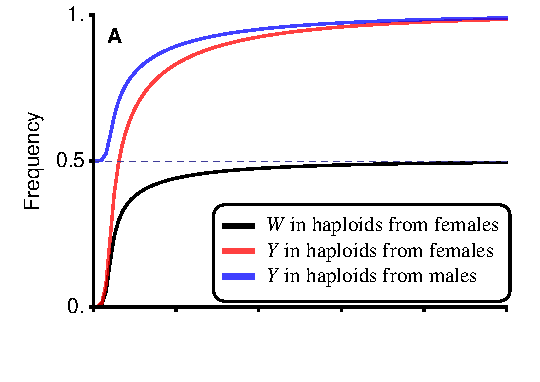
\includegraphics[width=0.5\linewidth]{FreqWLowR}\\
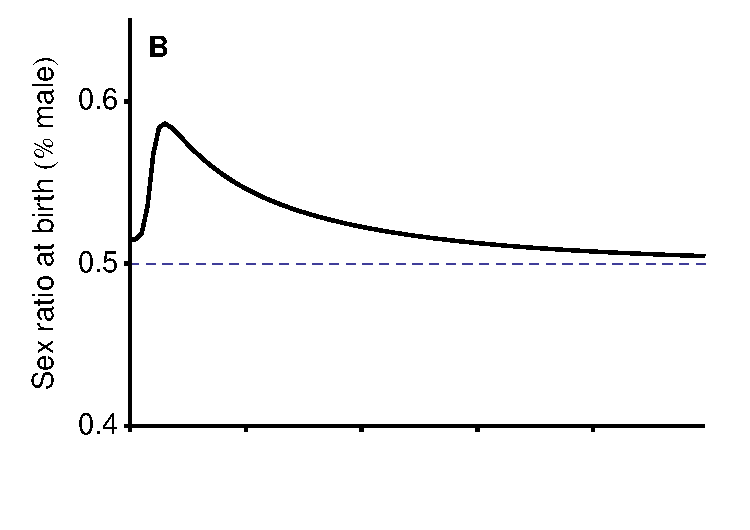
\includegraphics[width=0.5\linewidth]{SexRatioLowR}\\
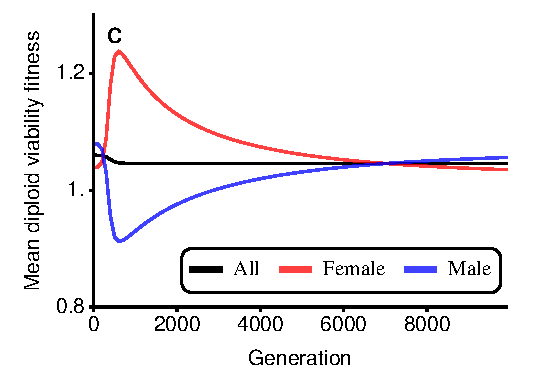
\includegraphics[width=0.5\linewidth]{MeanDipFitLowR}
\caption{
Haploid selection allows a neo-$W$ to invade an ancestral $XY$ system and fix (\textbf{A}) despite temporarily biasing the sex ratio further (\textbf{B}) and decreasing mean diploid viability fitness (\textbf{C}).
Complete turnover between genetic sex-determination systems occurs despite the neo-$W$ being less tightly linked to the selected locus than the ancestral sex-determining locus is, $R>r$.
Parameters: $k=1$, $s^f = 0.05$, $s^m = 0.15$, $h^f = h^m = 0.7$, $t^f = 0$, $t^m = -0.1$, $\alpha^m = \alpha^f = 1/2$, $r=0.01$, $R=0.05$.
}
\label{fig:WinvasionLowR}
\end{figure}
%%%%%%%%%%%%%%%%%%%%%%%%%%%%%%%%%%%%%%%%%%%%%%%%%%%%%%%%%

%%%%%%%%%%%%%%%%%%%%%%%%%%%%%%%%%%%%%%%%%%%%%%%%%%%%%%%%%
%W invades XY but does not fix
%%%%%%%%%%%%%%%%%%%%%%%%%%%%%%%%%%%%%%%%%%%%%%%%%%%%%%%%%
\begin{figure}
\centering
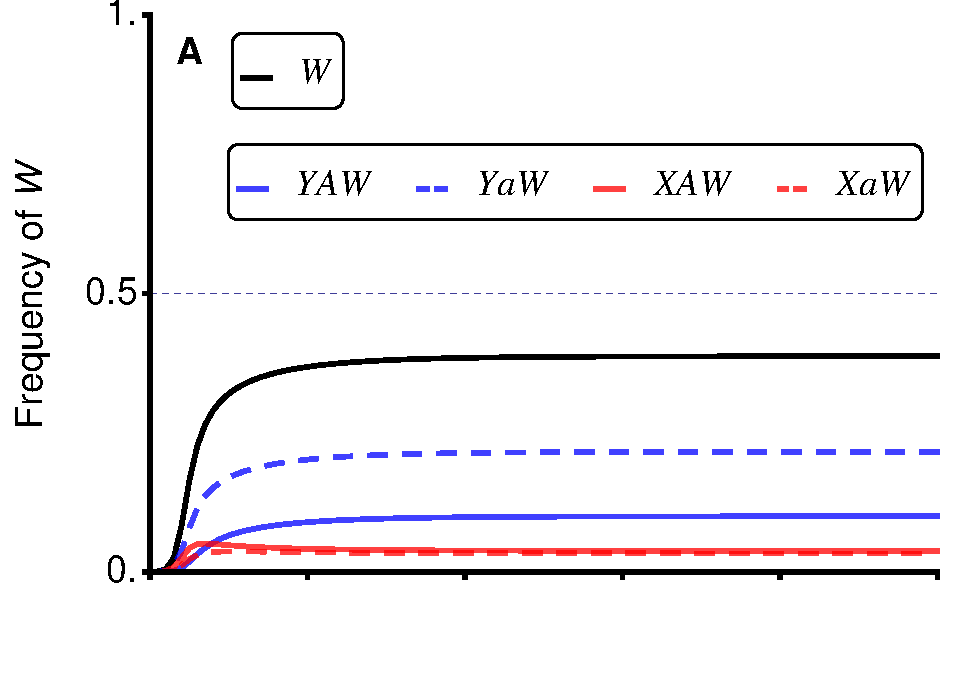
\includegraphics[width=0.5\linewidth]{FreqWHighR}\\
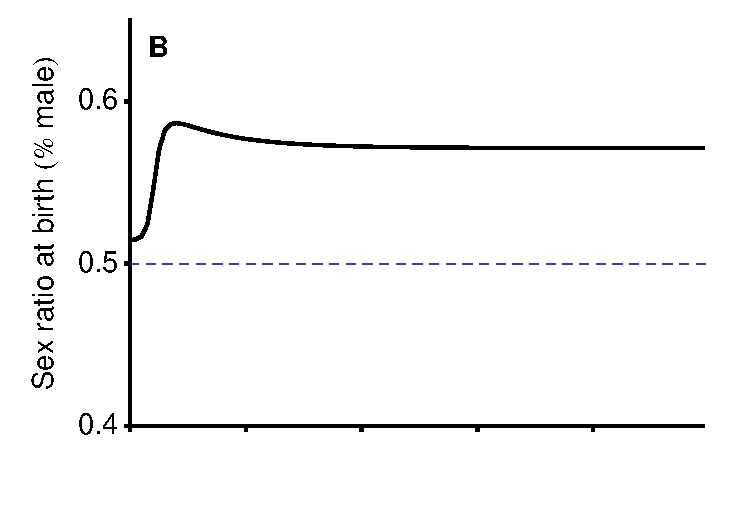
\includegraphics[width=0.5\linewidth]{SexRatioHighR}\\
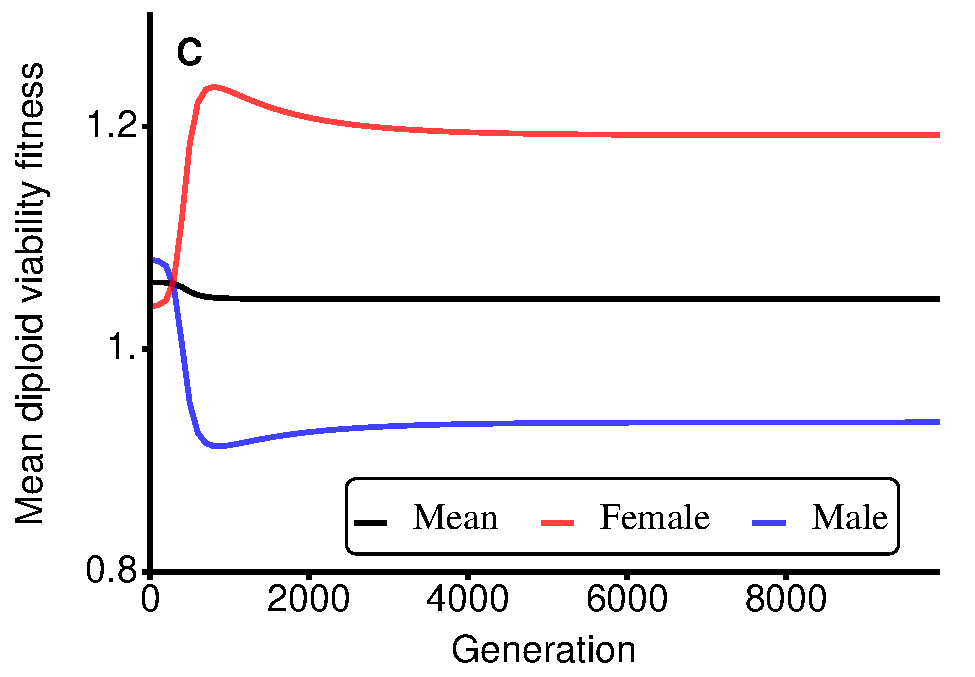
\includegraphics[width=0.5\linewidth]{MeanDipFitHighR}
\caption{
Haploid selection allows a completely unlinked neo-$W$ to invade an ancestral $XY$ system (\textbf{A}) despite further biasing the sex ratio (\textbf{B}) and decreasing mean diploid viability fitness (\textbf{C}).
The neo-$W$ does not fix (although variation at the \textbf{A} locus is maintained, $V_A>0$), resulting in a polymorphic sex-determination system.
Parameters as in Figure \ref{fig:WinvasionLowR} but with $R=0.5$.
}
\label{fig:WinvasionHighR}
\end{figure}
%%%%%%%%%%%%%%%%%%%%%%%%%%%%%%%%%%%%%%%%%%%%%%%%%%%%%%%%%

%%%%%%%%%%%%%%%%%%%%%%%%%%%%%%%%%%%%%%%%%%%%%%%%%%%%%%%%%
%W invades for all rates of recombination with selected locus
%%%%%%%%%%%%%%%%%%%%%%%%%%%%%%%%%%%%%%%%%%%%%%%%%%%%%%%%%
%\begin{figure}
%\centering
%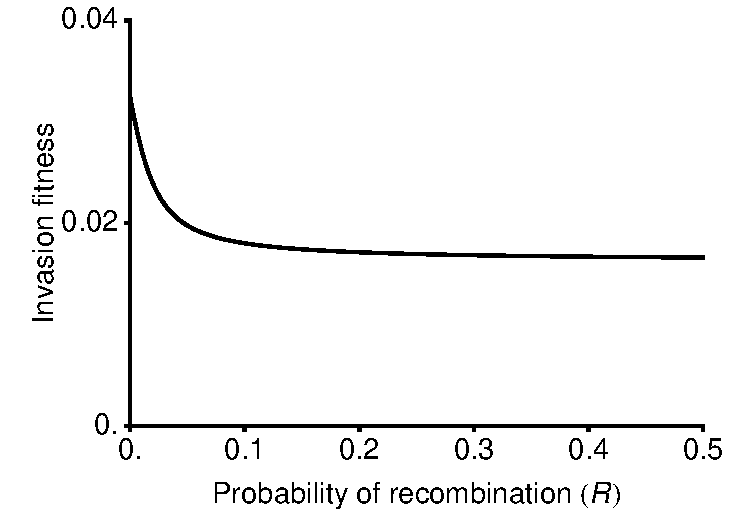
\includegraphics[width=0.5\linewidth]{InvasionVsRecombination}
%\caption{
%A neo-$W$ invades an ancestral $XY$ system with haploid selection regardless of how tightly it is linked to the selected locus. 
%Parameters as in Figure \ref{fig:WinvasionLowR}.
%}
%\label{fig:InvasionVsRecombination}
%\end{figure}
%%%%%%%%%%%%%%%%%%%%%%%%%%%%%%%%%%%%%%%%%%%%%%%%%%%%%%%%%

%%%%%%%%%%%%%%%%%%%%%%%%%%%%%%%%%%%%%%%%%%%%%%%%%%%%%%%%%
%W invasion versus position of selected locus
%%%%%%%%%%%%%%%%%%%%%%%%%%%%%%%%%%%%%%%%%%%%%%%%%%%%%%%%%
\begin{figure}
\centering
%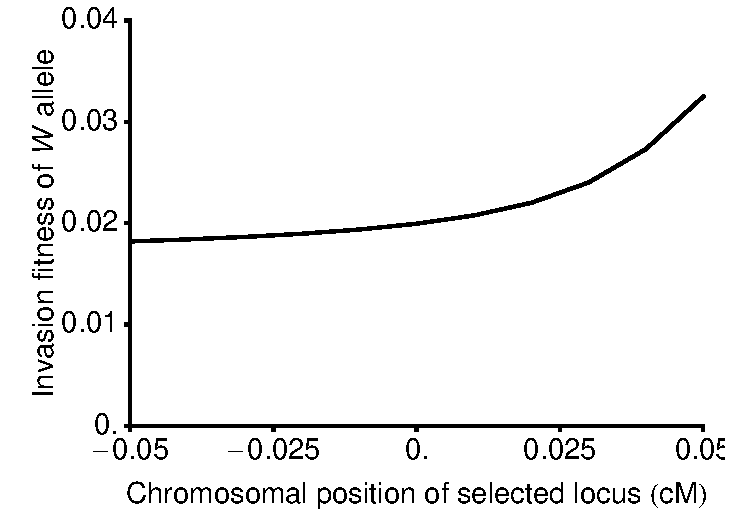
\includegraphics[width=0.5\linewidth]{InvasionVsCentiMorgans}
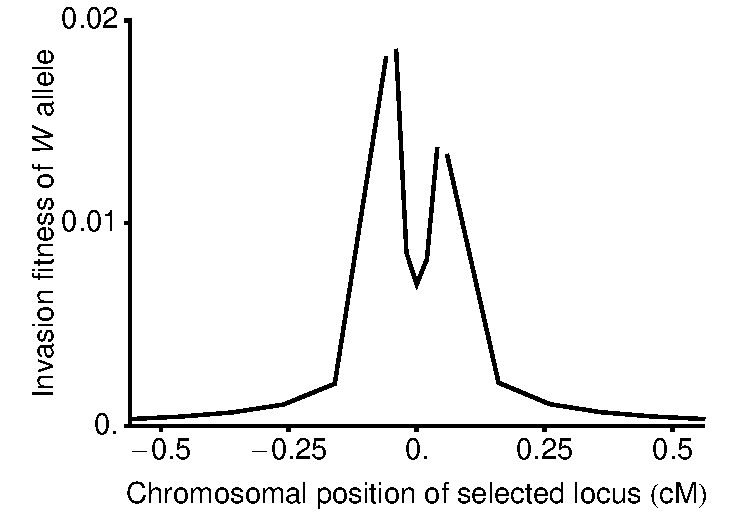
\includegraphics[width=0.5\linewidth]{InvasionVsCentiMorgansAllOrders}
\caption{
Haploid selection allows a neo-$W$ to invade an ancestral $XY$ system regardless of how tightly it and the ancestral sex-determining locus are linked to the selected locus. 
The ancestral sex-determining locus is located at -0.05 and the novel sex-determining locus is located at 0.05 (corresponding to the peaks of invasion fitness), such that the probability of a cross-over between them is $\approx0.1$.
The x-axis gives the position of the locus under haploid selection.
We used Haldane's map function \citep[Equation 3 in ][]{Haldane1919} to convert from map distance (centiMorgans) to the probability of a cross-over event. 
Parameters as in Figure \ref{fig:WinvasionLowR}.
}
\label{fig:InvasionVsCentiMorgans}
\end{figure}
%%%%%%%%%%%%%%%%%%%%%%%%%%%%%%%%%%%%%%%%%%%%%%%%%%%%%%%%%

%%%%%%%%%%%%%%%%%%%%%%%%%%%%%%%%%%%%%%%%%%%%%%%%%%%%%%%%%
%Y invades ZW and fixes (counter example to Kozi explanation)
%%%%%%%%%%%%%%%%%%%%%%%%%%%%%%%%%%%%%%%%%%%%%%%%%%%%%%%%%
\begin{figure}
\centering
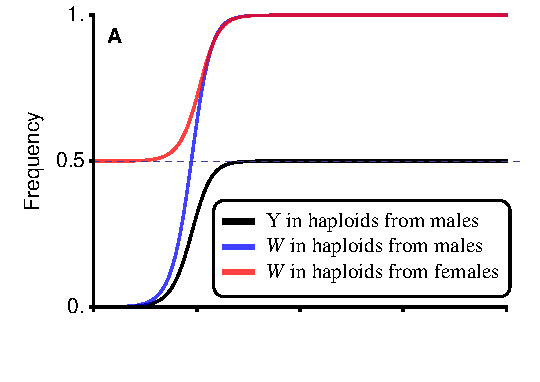
\includegraphics[width=0.5\linewidth]{FreqWCounterKozi}\\
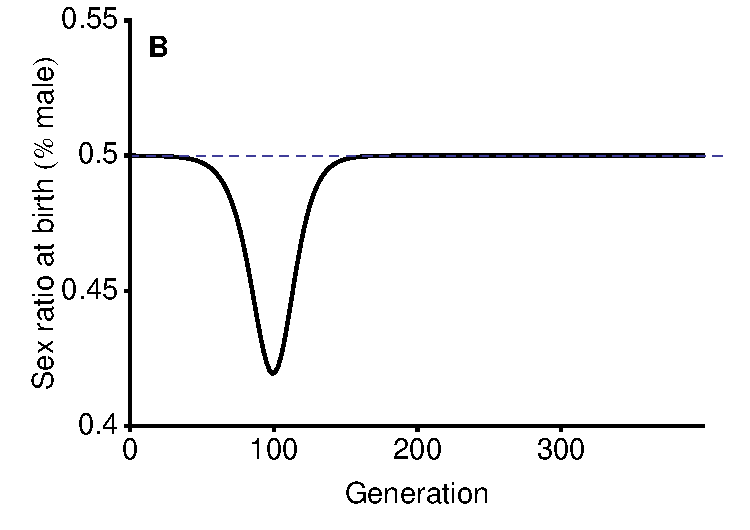
\includegraphics[width=0.5\linewidth]{SexRatioCounterKozi}\\
%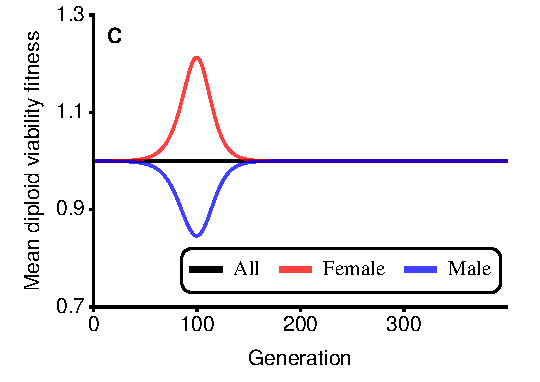
\includegraphics[width=0.5\linewidth]{MeanDipFitCounterKozi}
\caption{
Meiotic drive allows a neo-$Y$ to invade an ancestral $ZW$ system and fix (\textbf{A}) despite temporarily biasing the sex ratio (\textbf{B}). %and decreasing mean diploid viability fitness (\textbf{C}).
Parameters: $k=0$, $s^f = s^m = t^f = t^m = 0$, $\alpha^m = 0.4$, $\alpha^f = 1/2$, $r=0$, $R=0$.
}
\label{fig:CounterKozi}
\end{figure}
%%%%%%%%%%%%%%%%%%%%%%%%%%%%%%%%%%%%%%%%%%%%%%%%%%%%%%%%%














\setcounter{equation}{0}
\renewcommand{\theequation}{S.\arabic{equation}}
\setcounter{figure}{0}
\renewcommand{\thefigure}{S.\arabic{figure}}
\setcounter{table}{0}
\renewcommand{\thetable}{S.\arabic{table}}

%%%%%%%%%%%%%%%%%%%%%%%%%%%%%%%%%%%%%%%%%%%%%%%%%%%%%%%%%
\newpage

\section*{Appendix}

\subsection*{Recursion Equations}
\label{app:recurs}

In each generation we census the genotype frequencies in male and female gametes/gametophytes (hereafter, gametes) before haploid competition. 
Before haploid competition, the frequencies of X-bearing male and female gametes are given by $X_{i}^{m}$ and $X_{i}^{f}$ and the frequencies of Y-bearing gametes are given by $Y_{i}^{m}$ and $Y_{i}^{f}$ where the index $i$ specifies genotypes $MA=1$, $Ma=2$, $mA=3$, and $ma=4$. 
Competition then occurs among gametes of the same sex (e.g., among eggs and among sperm separately) according to the \textbf{A} locus allele, $g$ ($g\in A$, $a$, see Table \ref{tab:fitnesstable}), carried by individuals with genotype $i$.
The genotype frequencies after haploid competition are $X_{i}^{d,s}= w_{g}X_{i}^{d}/\bar{w}_{H}^{d}$ and $Y_{i}^{d,s}= w_{g}Y_{i}^{d}/\bar{w}_{H}^{d}$, where $\bar{w}_{H}^{d}=\sum_{i=1}^{4} w_{g}X_{i}^{d}+w_{g}Y_{i}^{d}$ is the mean fitness of male ($d=m$) or female ($d=f$) gametes. 
Random mating then occurs between gametes to produce diploid zygotes with genotype $ij$ at the \textbf{A} and \textbf{M} loci, such that $XX$ zygotes are denoted $xx_{ij}$, $XY$ zygotes are $xy_{ij}$, and $YY$ zygotes are $yy_{ij}$. 
In $XX$ and $YY$ zygotes, individuals with genotype $ij$ are equivalent to those with genotype $ji$. 
For simplicity, we denote the frequency of genotype $ij$ in $XX$ and $YY$ zygotes to the average of these frequencies, $xx_{ij}=(X_{i}^{f,s}X_{j}^{m,s}+X_{j}^{f,s}X_{i}^{m,s})/2$ and $yy_{ij}=(Y_{i}^{f,s}Y_{j}^{m,s}+Y_{j}^{f,s}Y_{i}^{m,s})/2$. 

Denoting the \textbf{M} locus genotype by $b$ ($b\in MM$, $Mm$, $mm$) and the \textbf{X} locus genotype by $c$ ($c\in XX$, $XY$, $YY$), zygotes develop as females with probability $k_{bc}$. 
Therefore, the frequencies of $XX$ females are given by $xx_{ij}^{f}=k_{bc}xx_{ij}$, $XY$ females are given by $xy_{ij}^{f}=k_{bc}xy_{ij}$, and $YY$ females are given by $yy_{ij}^{f}=k_{bc}xy_{ij}$. 
Similarly, $XX$ male frequencies are $xx_{ij}^{m}=(1-k_{bc})xx_{ij}$, $XY$ male frequencies are $xy_{ij}^{m}=(1-k_{bc})xy_{ij}$, and $YY$ males frequencies are $yy_{ij}^{m}=(1-k_{bc})xy_{ij}$.
This notation allows both the ancestral and novel sex-determining regions to determine zygotic sex according to an $XY$ system, a $ZW$ system, or an environmental sex-determining system. 
In addition, we can consider any dominance relationship between the two sex-determining loci. 
Typically, we assume that the ancestral sex-determining system (\textbf{X} locus) is $XY$ ($k_{MMXX}=1$ and $k_{MMXY}=k_{MMYY}=0$) and recessive to a dominant novel sex-determining locus, \textbf{M} ($k_{Mmc}=k_{mmc}=k$). 


Selection among diploids then occurs according to the diploid genotype at the \textbf{A} locus, $h$, for an individual of type $ij$ ($h \in AA$, $Aa$, $aa$, see Table \ref{tab:fitnesstable}). 
The diploid frequencies after selection in sex $d$ are given by $xx_{ij}^{d,s}=w_{h}^{d} xx_{ij}/\bar{w}^{d}$, $xy_{ij}^{d,s}=w_{h}^{d} xy_{ij}/\bar{w}^{d}$, and $yy_{ij}^{d,s}=w_{h}^{d} yy_{ij}/\bar{w}^{d}$, where $\bar{w}^{d}= \sum_{i=1}^{4}\sum_{j=1}^{4}w_{h}^{d}xx_{ij}+w_{h}^{d}xy_{ij}+w_{h}^{d}yy_{ij}$ is the mean fitness of individuals of sex $d$. 

Finally, these diploids undergo meiosis to produce the next generation of gametes. 
Recombination and sex-specific meiotic drive occur during meiosis.
%We can also assume that recombination is sex specific and/or affected by the M locus - but generally we don't so I just describe $R=R_{f}=R, r_{MM,d}=r_{Mm,d}=r_{mm,d}=r, \chi_{m}=\chi_{f}=\chi$.
Here, we allow the relative locations of the SDR, \textbf{A}, and \textbf{M} loci to be generic by using three parameters to describe the recombination rates between them. $R$ is the recombination rate between the \textbf{A} locus and the \textbf{M} locus, $\chi$ is the recombination rate between the \textbf{M} locus and the \textbf{X} locus, and $r$ is the recombination rate between the \textbf{A} locus and the \textbf{X} locus. 
Table \ref{tab:chisubstitutions} gives substitutions for $\chi$ for defined relative locations of these loci.
During meiosis in sex $d$, meiotic drive occurs such that, in $Aa$ heterozygotes, a fraction $\alpha_{d}$ of gametes produced carry the $A$ allele and $(1-\alpha^d)$ carry the $a$ allele. 

\begin{table}[ht]
\centering
\smallskip
\caption{$\chi$ substitutions for different loci orders (assuming no interference)}
\begin{tabular}{l l}
\hline\hline
  Order of loci &   \\ [0.5ex] \hline
  SDR-A-M & $\chi=R(1-r)+r(1-R)$  \\
  SDR-M-A & $\chi=(r-R)/(1-2R)$ \\
  A-SDR-M & $\chi=(R-r)/(1-2r)$ \\
  \hline \hline
  \label{tab:chisubstitutions}
 \end{tabular}
\end{table}

Among gametes from sex $d$ (sperm/pollen when $d=m$, eggs/ovules when $d=f$), the frequency of haplotypes (before haploid competition) in the next generation are given by

\begin{subequations}
\begin{equation}
\begin{split}
X_{MA}^{d'}=&xx_{11}^{d,s}+xx_{13}^{d,s}/2+(xx_{12}^{d,s}+xx_{14}^{d,s})\alpha^d\\
&-R(xx_{14}^{d,s}-xx_{23}^{d,s}) \alpha^d\\
&+(xy_{11}^{d,s}+xy_{13}^{d,s})/2+(xy_{12}^{d,s}+xy_{14}^{d,s})\alpha^d\\
&- r(xy_{12}^{d,s}-xy_{21}^{d,s})\alpha^d - \chi(xy_{13}^{d,s}-xy_{31}^{d,s})/2\\
&+\big{\{}-(R+r+\chi)xy_{14}^{d,s} +(r+\chi-R)xy_{41}^{d,s}\\
&+(R+r-\chi) xy_{23}^{d,s}+(R+\chi-r)xy_{32}^{d,s}\big{\}}\alpha^d/2
\end{split}
\end{equation}
%
\begin{equation}
\begin{split}
X_{Ma}^{d'}=&xx_{22}^{d,s}+xx_{24}^{d,s}/2+(xx_{12}^{d,s}+xx_{23}^{d,s})\alpha^d\\
&-R(xx_{23}^{d,s}-xx_{14}^{d,s}) \alpha^d\\
&(xy_{22}^{d,s}+xy_{24}^{d,s})/2+(xy_{21}^{d,s}+xy_{23}^{d,s})(1-\alpha^d)\\
&- r(xy_{21}^{d,s}-xy_{12}^{d,s})(1-\alpha^d) - \chi(xy_{24}^{d,s}-xy_{42}^{d,s})/2\\
&+\big{\{}-(R+r+\chi)xy_{23}^{d,s}+(r+\chi-R)xy_{32}^{d,s}\\
&+(R+r-\chi) xy_{14}^{d,s}+(R+\chi-r)xy_{41}^{d,s}\big{\}}(1-\alpha^d)/2
\end{split}
\end{equation}
%
\begin{equation}
\begin{split}
X_{mA}^{d'}=&xx_{33}^{d,s}+xx_{13}^{d,s}/2+(xx_{23}^{d,s}+xx_{34}^{d,s})\alpha^d\\
&-R(xx_{23}^{d,s}-xx_{14}^{d,s}) \alpha^d\\
&(xy_{33}^{d,s}+xy_{31}^{d,s})/2+(xy_{32}^{d,s}+xy_{34}^{d,s})\alpha^d\\
&- r(xy_{34}^{d,s}-xy_{43}^{d,s}) \alpha^d - \chi(xy_{31}^{d,s}-xy_{13}^{d,s})/2\\
&+\big{\{}-(R+r+\chi)xy_{32}^{d,s} +(r+\chi-R)xy_{23}^{d,s}\\
&+(R+r-\chi) xy_{41}^{d,s}+(R+\chi-r)xy_{14}^{d,s}\big{\}} \alpha^d/2
\end{split}
\end{equation}
%
\begin{equation}
\begin{split}
X_{ma}^{d'}=&xx_{44}^{d,s}+xx_{34}^{d,s}/2+(xx_{14}^{d,s}+xx_{24}^{d,s})\alpha^d\\
&-R(xx_{14}^{d,s}-xx_{23}^{d,s}) \alpha^d\\
&(xy_{44}^{d,s}+xy_{42}^{d,s})/2+(xy_{41}^{d,s}+xy_{43}^{d,s})(1-\alpha^d)\\
&- r(xy_{43}^{d,s}-xy_{34}^{d,s})(1-\alpha^d) - \chi(xy_{42}^{d,s}-xy_{24}^{d,s})/2\\
&+\big{\{}-(R+r+\chi)xy_{41}^{d,s}+(r+\chi-R)xy_{14}^{d,s}\\
&+(R+r-\chi) xy_{32}^{d,s}+(R+\chi-r)xy_{23}^{d,s}\big{\}}(1-\alpha^d)/2
\end{split}
\end{equation}
%%%%%%%%%%%%%%%%%%%
%
\begin{equation}
\begin{split}
Y_{MA}^{d'}=&yy_{11}^{d,s}+yy_{13}^{d,s}/2+(yy_{12}^{d,s}+yy_{14}^{d,s})\alpha^d\\
&-R(yy_{14}^{d,s}-yy_{23}^{d,s}) \alpha^d\\
&(xy_{11}^{d,s}+xy_{31}^{d,s})/2+(xy_{21}^{d,s}+xy_{41}^{d,s})\alpha^d\\
&- r(xy_{21}^{d,s}-xy_{12}^{d,s})\alpha^d - \chi(xy_{31}^{d,s}-xy_{13}^{d,s})/2\\
&+\big{\{} - (R+r+\chi)xy_{41}^{d,s} + (r+\chi-R)xy_{14}^{d,s}\\
& + (R+r-\chi)xy_{32}^{d,s} + (R+\chi-r) xy_{23}^{d,s}\big{\}}\alpha^d/2
\end{split}
\end{equation}
%
\begin{equation}
\begin{split}
Y_{Ma}^{d'}=&yy_{22}^{d,s}+yy_{24}^{d,s}/2+(yy_{12}^{d,s}+yy_{23}^{d,s})\alpha^d\\
&-R(yy_{23}^{d,s}-yy_{14}^{d,s}) \alpha^d\\
&(xy_{22}^{d,s}+xy_{42}^{d,s})/2+(xy_{12}^{d,s}+xy_{32}^{d,s})(1-\alpha^d)\\
&- r(xy_{12}^{d,s}-xy_{21}^{d,s})(1-\alpha^d) - \chi(xy_{42}^{d,s}-xy_{24}^{d,s})/2\\
&+\big{\{}-(R+r+\chi)xy_{32}^{d,s} +(r+\chi-R) xy_{23}^{d,s}\\
&+(R+r-\chi)xy_{41}^{d,s}+(R+\chi-r)xy_{14}^{d,s}\big{\}}(1-\alpha^d)/2
\end{split}
\end{equation}
%
\begin{equation}
\begin{split}
Y_{mA}^{d'}=&yy_{33}^{d,s}+yy_{13}^{d,s}/2+(yy_{23}^{d,s}+yy_{34}^{d,s})\alpha^d\\
&-R(yy_{23}^{d,s}-yy_{14}^{d,s}) \alpha^d\\
&(xy_{33}^{d,s}+xy_{13}^{d,s})/2+(xy_{23}^{d,s}+xy_{43}^{d,s})\alpha^d\\
&- r(xy_{43}^{d,s}-xy_{34}^{d,s})\alpha^d - \chi(xy_{13}^{d,s}-xy_{31}^{d,s})/2\\
&+\big{\{}-(R+r+\chi)xy_{23}^{d,s} +(r+\chi-R)xy_{32}^{d,s}\\
&+(R+r-\chi) xy_{14}^{d,s} + (R+\chi-r) xy_{41}^{d,s}\big{\}}\alpha^d/2
\end{split}
\end{equation}
%
\begin{equation}
\begin{split}
Y_{ma}^{d'}=&yy_{44}^{d,s}+yy_{34}^{d,s}/2+(yy_{14}^{d,s}+yy_{24}^{d,s})\alpha^d\\
&-R(yy_{14}^{d,s}-yy_{23}^{d,s}) \alpha^d\\
&(xy_{44}^{d,s}+xy_{24}^{d,s})/2+(xy_{14}^{d,s}+xy_{34}^{d,s})(1-\alpha^d)\\
&- r(xy_{34}^{d,s}-xy_{43}^{d,s})(1-\alpha^d) - \chi(xy_{24}^{d,s}-xy_{42}^{d,s})/2\\
&+\big{\{}-(R+r+\chi) xy_{14}^{d,s} + (r+\chi-R)xy_{41}^{d,s}\\
&+(R+r-\chi) xy_{23}^{d,s} + (R+\chi-r) xy_{32}^{d,s}\big{\}}(1-\alpha^d)/2
\end{split}
\end{equation}
\label{eq:recursions}
\end{subequations}

\noindent
The full system is therefore described by 16 recurrence equations (three loci, each with two alleles, and two gamete sexes yields 16 combinations). 
However, some diploid types are not produced under a given sex determination system. 
For example, with the $M$ allele fixed and ancestral $XY$ sex determination, there are no $XX$ males, $XY$ females, or $YY$ females ($xx_{11}^{m}$, $xx_{12}^{m}$, $xx_{22}^m$, $xy_{11}^{f}$, $xy_{12}^{f}$, $xy_{22}^f$, $yy_{11}^{f}$, $yy_{12}^{f}$, and $yy_{22}^f$ are all 0). 
In this case, the system only involves six recursion equations because there is only one \textbf{M} locus allele and no Y-bearing female gametes. 
This six-equation system yields equilibrium \eqref{eq:pAve}. 
Within this resident population (when $m$ is absent) we describe frequencies among different gamete types, which are given by $X_{MA}^{f}=p_{Xf}$, $X_{Ma}^{f}=(1-p_{Xf})$, $X_{MA}^{m}=(1-q)p_{Xm}$, $X_{Ma}^{m}=(1-q)(1-p_{Xm})$, $Y_{MA}^{m}=q p_{Ym}$, and $Y_{Ma}^{m}=q(1-p_{Ym})$.

\end{document}



